\documentclass{article}
\usepackage{amsmath, amssymb, tikz}
\begin{document}

\title{A Derivation of the Cosine Rule}
\author{Tutoring Centre Ferndale\\

\includegraphics[width=4em]{ApS_logo.png}}
\date{}
\begin{document}
\maketitle

The cosine rule relates the lengths of the sides of a triangle to the cosine of one of its angles. Given a triangle $\triangle ABC$ with sides labeled as follows:

\begin{itemize}
    \item $a$ is the length of side $BC$, opposite angle $A$.
    \item $b$ is the length of side $AC$, opposite angle $B$.
    \item $c$ is the length of side $AB$, opposite angle $C$.
\end{itemize}

The cosine rule states:
\[
c^2 = a^2 + b^2 - 2ab \cos C.
\]
We derive this formula using trigonometry and the Pythagorean theorem.

Dropping a perpendicular from vertex $C$ to the base $AB$, meeting it at point $D$ creates two right-angled triangles $\triangle ADC$ and $\triangle BDC$.

\begin{itemize}
    \item $AD = x$: the part of $AB$ on the left.
    \item $DB = c - x$: the remaining part of $AB$.
    \item $CD = h$: the height of the triangle.
\end{itemize}

Thus, $\triangle ADC$ has hypotenuse $b$, and $\triangle BDC$ has hypotenuse $a$.

\begin{center}
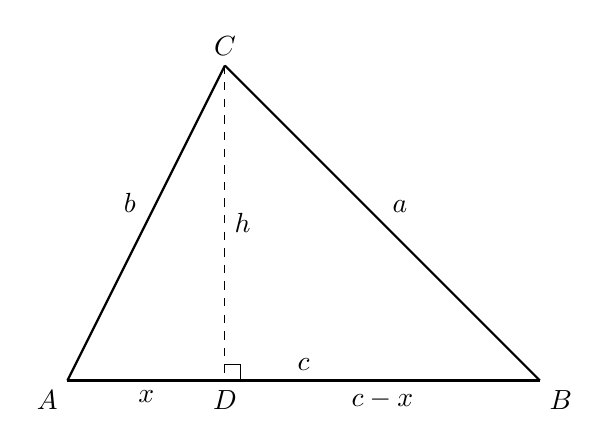
\begin{tikzpicture}
    % Define points
    \coordinate (A) at (0,0);
    \coordinate (B) at (6,0);
    \coordinate (C) at (2,4);
    \coordinate (D) at (2,0);

    % Draw the triangle
    \draw [thick] (A) -- (B) node[midway,above]{$c$};
    \draw [thick] (B) -- (C) node[midway,above right]{$a$};
    \draw [thick] (C) -- (A) node[midway,above left]{$b$};
    
    % Draw the height
    \draw [dashed] (C) -- (D);
    
    % Mark the right angle
    \draw (D) ++(0.2,0) -- ++(0,0.2) -- ++(-0.2,0);
    
    % Label vertices
    \node [below left] at (A) {$A$};
    \node [below right] at (B) {$B$};
    \node [above] at (C) {$C$};
    \node [below] at (D) {$D$};
    
    % Label height
    \node [right] at (2,2) {$h$};
    
    % Label segments on the base
    \node [below] at (1,0) {$x$};
    \node [below] at (4,0) {$c-x$};
    
\end{tikzpicture}
\end{center}

From $\triangle ADC$:
\begin{align*}
    \cos A &= \frac{x}{b} \Rightarrow x = b \cos A, \\
    \sin A &= \frac{h}{b} \Rightarrow h = b \sin A.
\end{align*}

From $\triangle BDC$:
\begin{align*}
    \cos B &= \frac{c - x}{a} \Rightarrow c - x = a \cos B, \\
    \sin B &= \frac{h}{a} \Rightarrow h = a \sin B.
\end{align*}

Since both expressions for $h$ must be equal:
\[
b \sin A = a \sin B.
\]
This is the sine rule, but we need to proceed further to derive the cosine rule.

Using Pythagoras' Theorem in $\triangle ADC$:
\begin{align*}
    h^2 + x^2 &= b^2.
\end{align*}
Substituting $h = b \sin A$ and $x = b \cos A$:
\begin{align*}
    (b \sin A)^2 + (b \cos A)^2 &= b^2, \\
    b^2 \sin^2 A + b^2 \cos^2 A &= b^2.
\end{align*}
Factoring out $b^2$:
\[
b^2 (\sin^2 A + \cos^2 A) = b^2.
\]\\
Using the identity $\sin^2 A + \cos^2 A = 1$:
\[
b^2 \cdot 1 = b^2.
\]
Thus, this equation holds true.\\

Now applying Pythagoras' Theorem in $\triangle BDC$:
\begin{align*}
    h^2 + (c - x)^2 &= a^2.
\end{align*}
Substituting $h = b \sin A$ and $c - x = a \cos B$:
\begin{align*}
    (b \sin A)^2 + (a \cos B)^2 &= a^2, \\
    b^2 \sin^2 A + a^2 \cos^2 B &= a^2.
\end{align*}
Expanding and rearranging:
\[
c^2 = a^2 + b^2 - 2ab \cos C.
\]
which is the desired cosine rule.

\end{document}
